\documentclass{scu-thesis}
\usepackage{amsmath}	% for advanced typesetting of mathematics
\usepackage{graphicx}	% for including graphics
\usepackage{natbib}	% for better citation styles
\usepackage{txfonts}	% for using the Times-Roman font


% These must be set first ... the rest of the thesis commands rely on them.

\author{Manoj Adhikari}
\author{Colby Harper}
\author{Sean Karstein}
\title{On the Construction of Matter, or Is There a God Particle?}
\department{Department of Computer Engineering}
\degree{Bachelor of Science in Computer Science and Engineering}


% Only bachelor's theses should have multiple authors and/or be from
% multiple departments.  Signatures required:
%
% Bachelor's theses: advisor(s), department chair(s)
% Master's theses: advisor, reader, department chair
% Doctoral theses: doctoral committee (including advisor), department chair

\begin{document}
\frontmatter
\signature{Thesis Advisor}
\signature{Thesis Advisor}
\signature{Department Chair}
\signature{Department Chair}

\maketitle
\begin{abstract}
Taking group photos during important events is a common practice. Group photos are taken to remember cheerful times when people had opportunity to meet many other people. However, an unappealing facial experience of one person can easily ruin the entire photo. Capturing the wrong moments when a person doesn't look attractive can leave him/her displeased from the complete event experience. A solution is to develop a mobile app that captures the moment when everyone is smiling with eyes wide open. Our solution aims to develop an iPhone app that will preclude users from worrying about not having a great group picture. 
\end{abstract}


\tableofcontents
\listoffigures

\mainmatter
\chapter{Introduction}
Taking pictures to save our best memories is a common practice. During group pictures, photos can be entirely ruined by a single person?s expressions. We all have seen photos of people who did not smile/looked away, or worse, been that person. The experiences at big events and gatherings would be much more fulfilling if we didn?t have to take many pictures just to get a nice smiling photo. Modern cameras and phones have beautiful design incorporated with advanced features. However, they have forgotten to address this pesky issue that would uplift everyone?s picture taking moment. 

Currently, the only group photo technology to be created is the automatic photo with timer.  The purpose of this is to eliminate the need for someone to click the button to take the photo, however it is not smart.  It does not signal when the photo will be taken, and takes the photo only when the timer has reached zero.  Therefore, this does not have any effect on the quality of the photo.  Currently, the only solutions affecting the quality of group photos are after effect softwares such as photoshop.  However, these often require a large amount of money, and a level of skill in using the product, which most people don?t have.

We propose to build an iOS app that utilizes the iPhone?s camera and adds the feature of taking pictures automatically when everyone in the group is looking at the camera with their eyes open and smiling. The app will automate the tedious task of capturing the right moment saving people?s time for actually enjoying the moment.  Computer vision will be used to narrow the focus of the image, to then allow a machine learning model to determine when the right moment to snap the photo is.

To conclude, our design will accomplish two things: firstly, it will save time for both people who are getting their photo taken as well as the person taking the photo, as the camera will know exactly when to take the right photo, and secondly, will improve the quality of photos, allowing for memories to be better cherished by all. 




\chapter{Requirements}

\section{Functional Requirements}
Critical:
\begin{itemize}
 \item Users can take pictures using iPhone camera.
 \item Users can choose to save or disregard the photo captured.
 \item The app can identify if everyone in the group is smiling with eyes wide open or not.
 \item Photos are automatically captured without users click.
 \end{itemize}
 
Recommended:
\begin{itemize}
\item Users can share pictures with their friends using phone numbers.
 \end{itemize}
 
Suggested:
\begin{itemize}
\item Users can give feedback on whether the app captured good pictures.
\item The system will offer photo editing features
 \end{itemize}
 
\section{Non-Functional Requirements}
Critical: 
\begin{itemize}
\item The user interface will be simple and intuitive 
\item The system will be easy to install and use.
 \end{itemize}
 
Recommended:
\begin{itemize}
\item The system will be secure from unauthorized users. 
 \end{itemize}
 
Suggested:
\begin{itemize}
\item The system will be high performance and will require minimal system resources.
 \end{itemize}
\section{Design Constraint}
\begin{itemize}
\item The app can only run on iPhones with iOS versions starting iOS  10.3.
 \end{itemize}


\chapter{Use Cases}
Use case diagrams demonstrate how users will interact with our system. In our case, users will be able to take photos, then accept or reject them. 

\begin{figure}[!h]
    \centering
    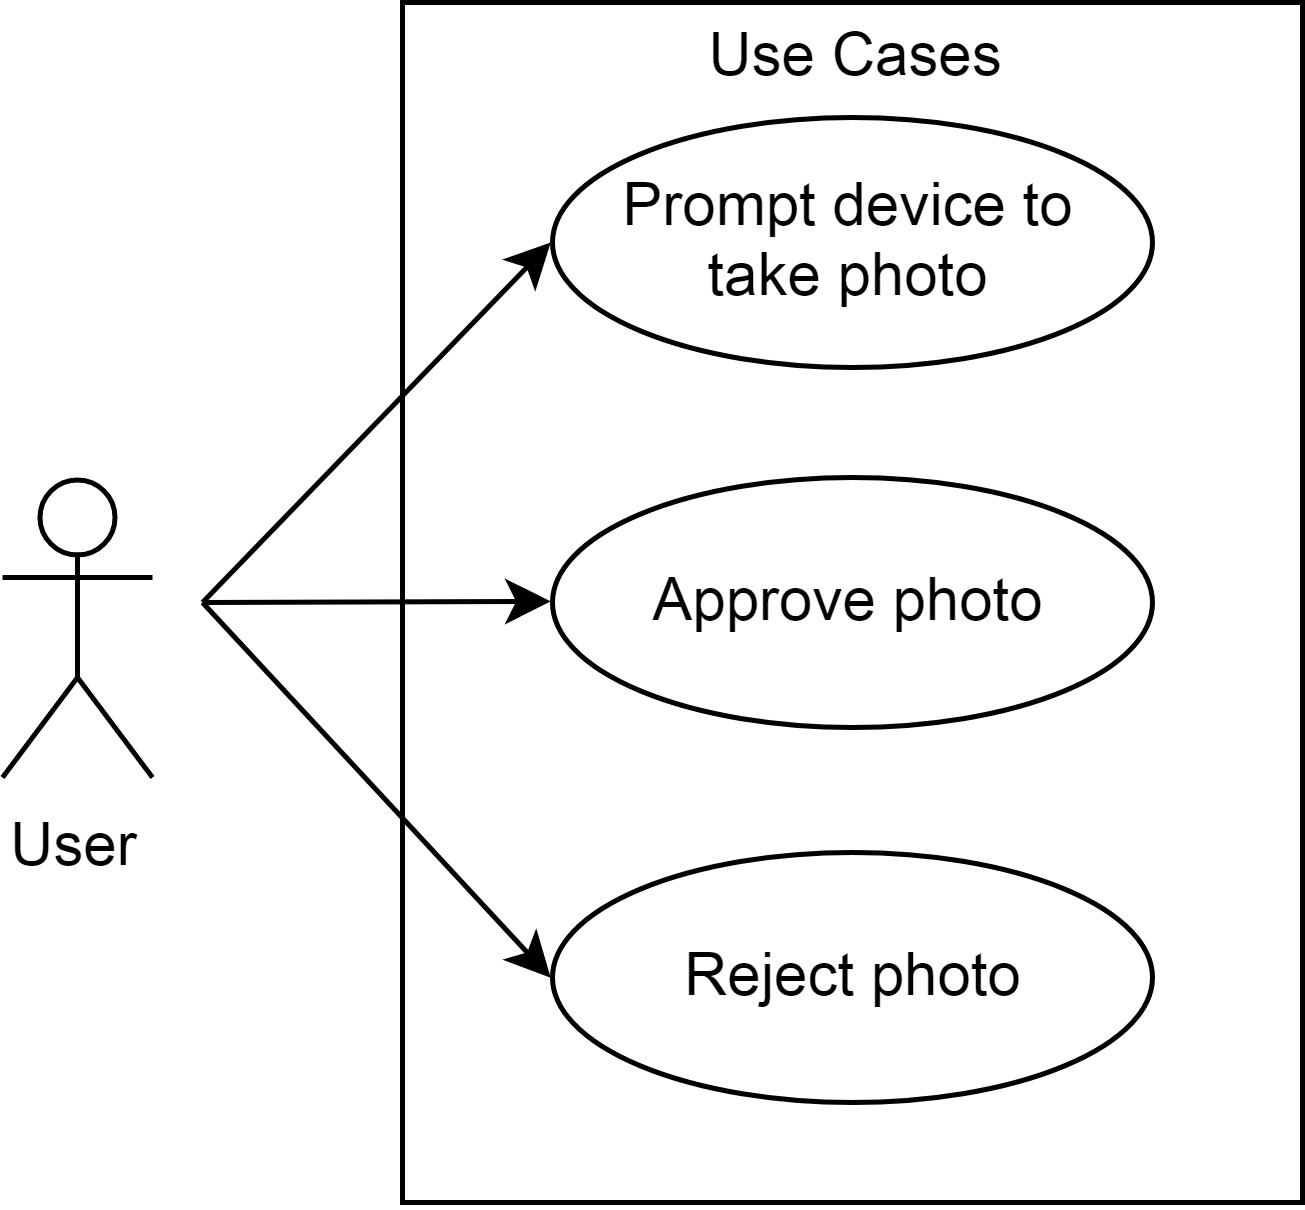
\includegraphics[scale=0.25]{usecasediagram}
    \caption{Use Cases}
    \label{fig:usecasediagram}
\end{figure}

\pagebreak

\begin{enumerate}
    \item Prompt device to take photo
    \begin{enumerate}
        \item Goal: Take photo
        \item Actors: User
        \item Pre-conditions:
            \begin{enumerate}
                \item Application must be open on device
            \end{enumerate}
        \item Steps:
            \begin{enumerate}
                \item User presses button to prompt device to take photo
            \end{enumerate}
        \item Post-conditions:
            \begin{enumerate}
                \item None
            \end{enumerate}
        \item Exceptions:
            \begin{enumerate}
                \item Application must have device permission to use camera
            \end{enumerate}
    \end{enumerate}
\end{enumerate}

\begin{enumerate}
    \item Approve photo
    \begin{enumerate}
        \item Goal: Save photo to phone storage
        \item Actors: User
        \item Pre-conditions:
            \begin{enumerate}
                \item Must have taken a photo
            \end{enumerate}
        \item Steps:
            \begin{enumerate}
                \item User presses accept button when prompted after taking a photo
            \end{enumerate}
        \item Post-conditions:
            \begin{enumerate}
                \item None
            \end{enumerate}
        \item Exceptions:
            \begin{enumerate}
                \item None
            \end{enumerate}
    \end{enumerate}
\end{enumerate}

\begin{enumerate}
    \item Reject photo
    \begin{enumerate}
        \item Goal: Delete photo and try again
        \item Actors: User
        \item Pre-conditions:
            \begin{enumerate}
                \item Must have taken a photo
            \end{enumerate}
        \item Steps:
            \begin{enumerate}
                \item User presses reject button when prompted after taking a photo
            \end{enumerate}
        \item Post-conditions:
            \begin{enumerate}
                \item None
            \end{enumerate}
        \item Exceptions:
            \begin{enumerate}
                \item None
            \end{enumerate}
    \end{enumerate}
\end{enumerate}



\chapter{Activity Diagram}

The flowchart outlines the workflow of all users actions and interactions with the system. The diagram does not show system actions, such as processing the image stream and deciding when to capture an image.

\begin{figure}[!h]
    \centering
    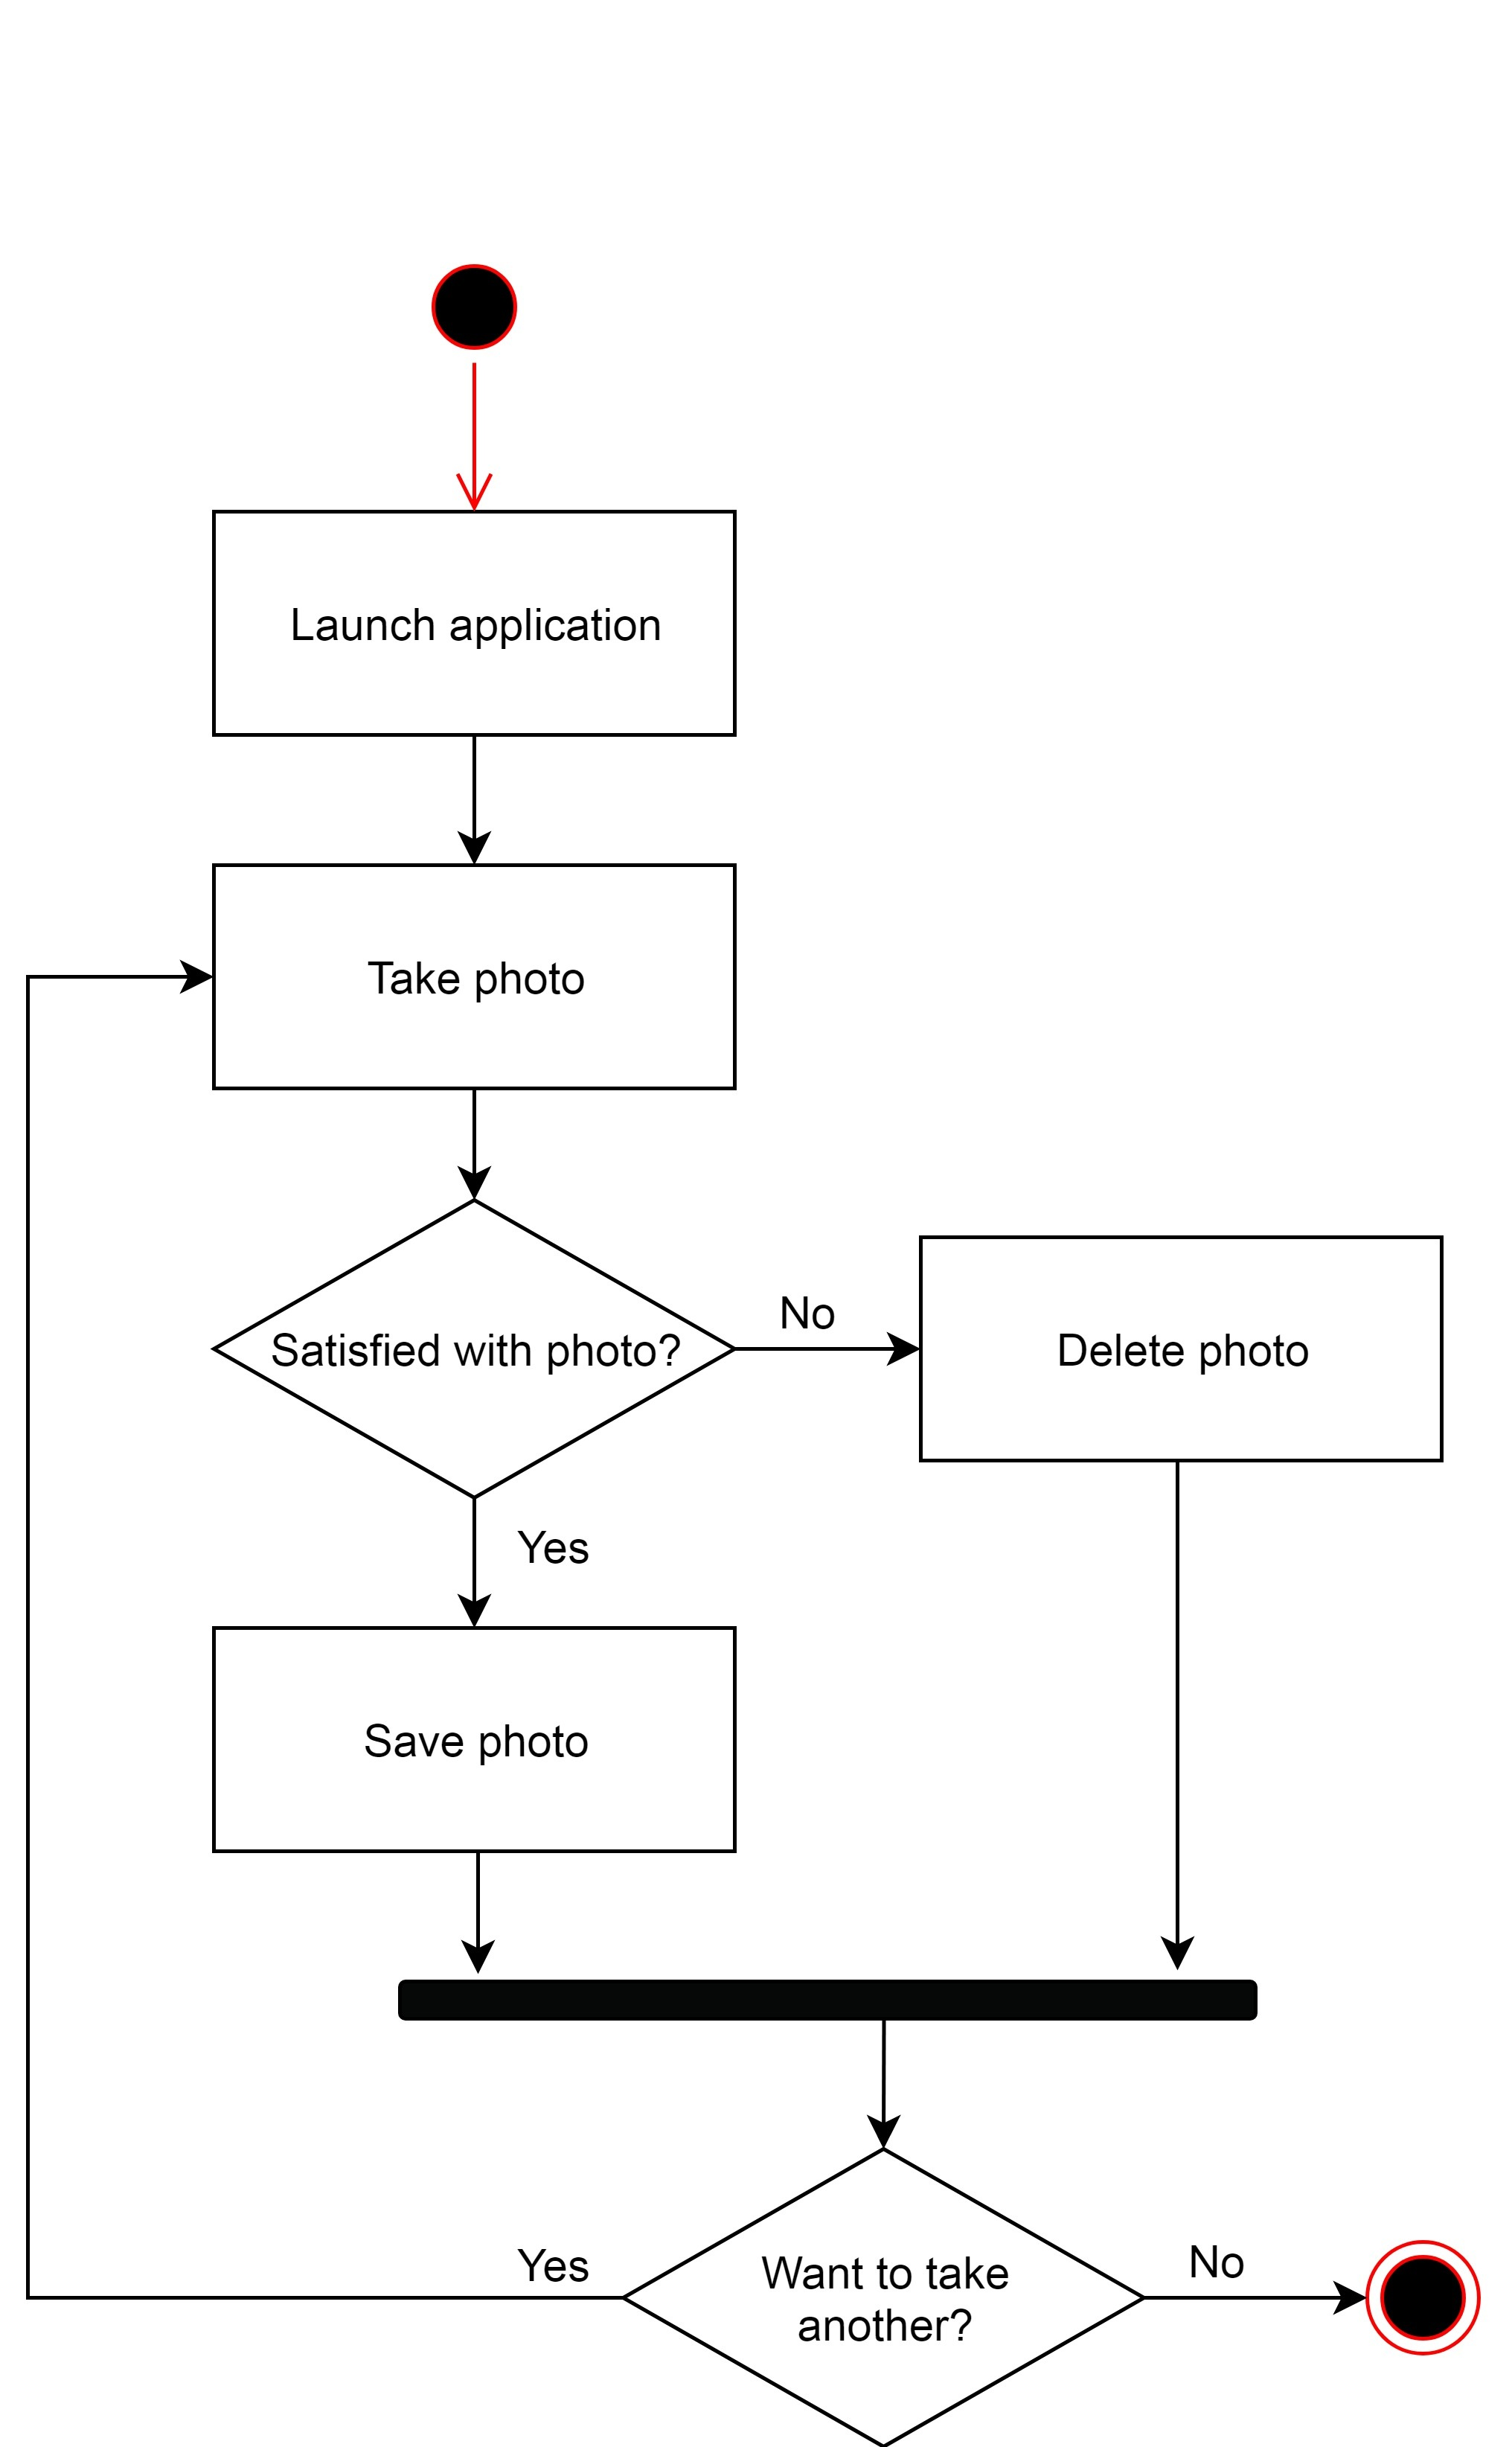
\includegraphics[width=0.75\textwidth]{activitydiagram}
    \caption{Figure 4.1: Work flow of user interacting with system}
    \label{fig:activitydiagram}
\end{figure}




\chapter{Conceptual Model}

Users will navigate to the application on an iPhone to begin using the system. Upon launching the app, a camera feed appears, as shown in Figure 5.1. They can press the camera icon to prompt the device to take a photo.

\begin{figure}[!h]
    \centering
    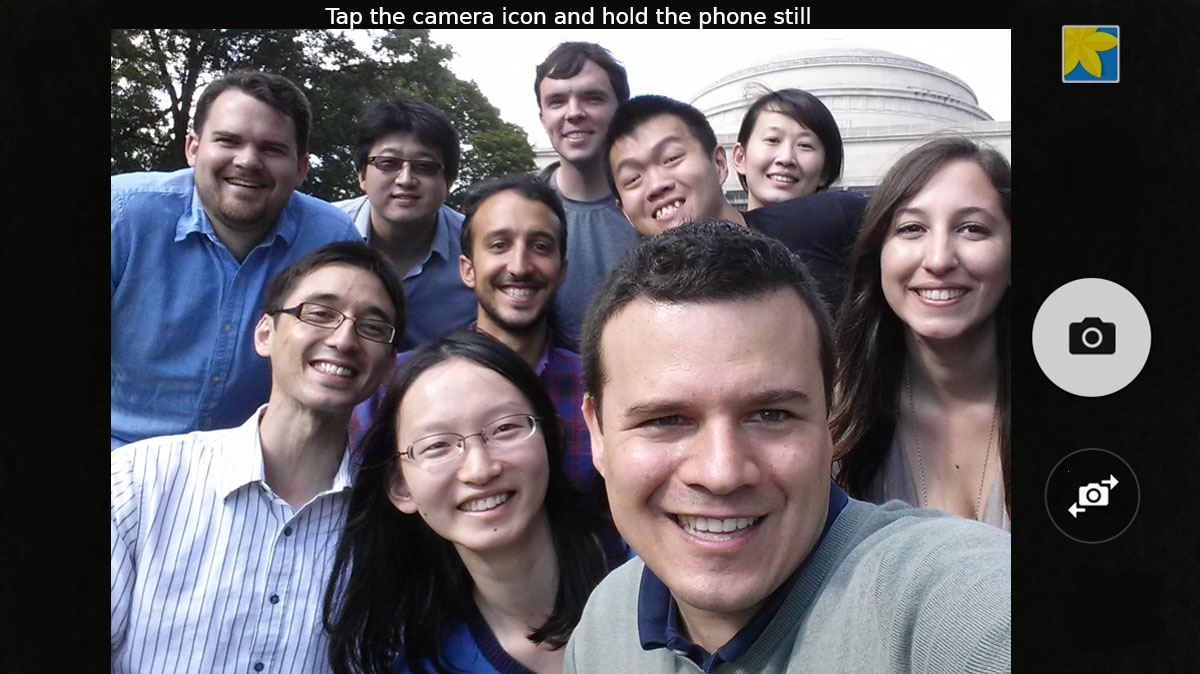
\includegraphics[width=0.75\textwidth]{conceptualmodel1}
    \caption{Mockup of camera user interface}
    \label{fig:conceptualmodel1}
\end{figure}

\pagebreak
After they has pressed the camera button, the application will wait until all subjects are in frame with their eyes open to capture the image. Upon capturing the image, they will be greeted with an alert asking whether they want to save the photo or reject it, as seen in Figure 5.2.

\begin{figure}[!h]
    \centering
    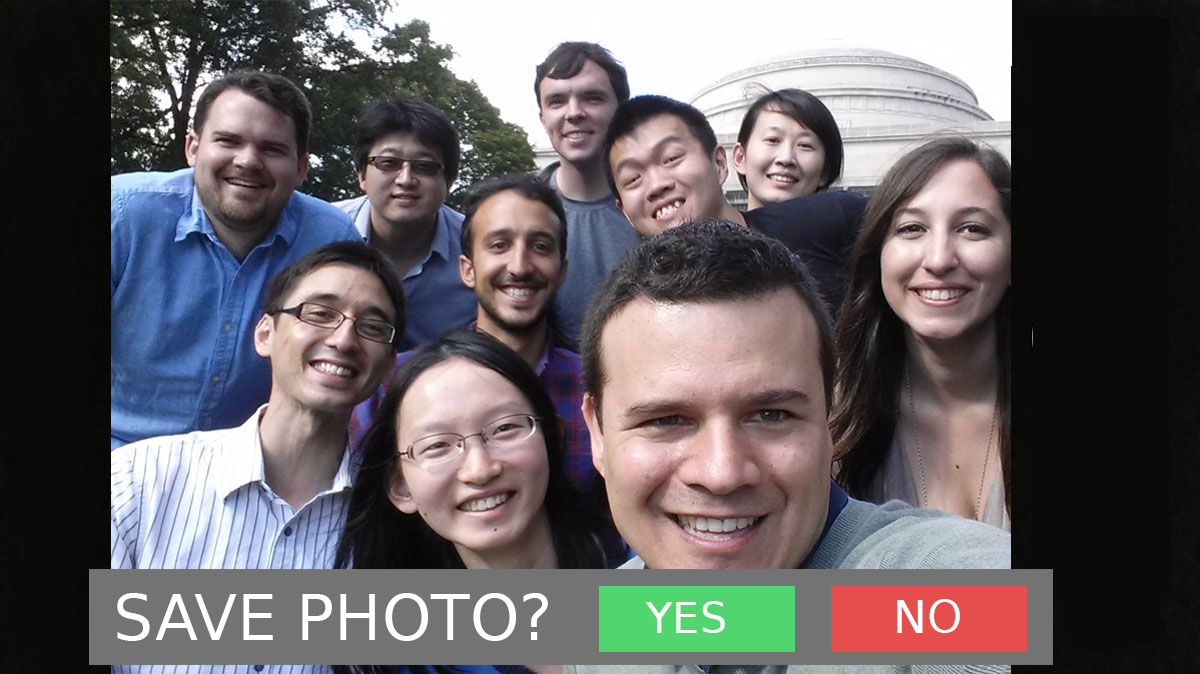
\includegraphics[width=0.75\textwidth]{conceptualmodel2}
    \caption{Mockup demonstrating the approval dialogue}
    \label{fig:conceptualmodel2}
\end{figure}

If the user chooses to accept the photo, then it will be saved to the user's storage and they will return to the camera screen. If the user chooses to discard the photo, then it will be delete and they will return to the camera.




\chapter{Architectural Diagram}

We plan to utilize a data flow architecture to complete this project as shown in Figure 6.1.

\begin{figure}[!h]
    \centering
    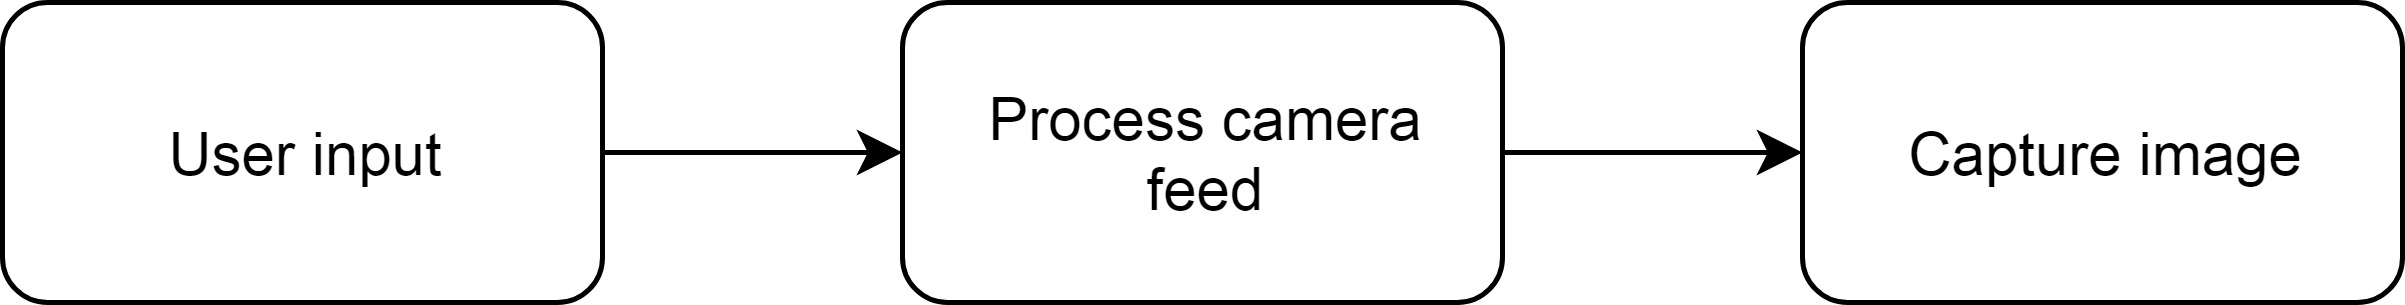
\includegraphics[width=0.75\textwidth]{architecturediagram}
    \caption{Figure 5.1: Data Flow Architecture}
    \label{fig:architecturediagram}
\end{figure}

Users will provide input with their phone's touchscreen, which triggers the device to begin analyzing the camera feed. Once the system determines the input is acceptable, it captures the image.



\chapter{Technologies Used}

\begin{itemize}
	\item Hardware
	\begin{itemize}
		\item Development
		\begin{itemize}
			\item Macbook Pro
			\item ThinkPad
		\end{itemize}
		\item Application Testing
			\begin{itemize}
				\item Iphone 7
				\item ThinkPad with Iphone emulator
			\end{itemize}
	\end{itemize}
	\item Programming Languages
	\begin{itemize}
		\item Swift
		\begin{itemize}
			\item For iOS Programming
		\end{itemize}
		\item Python
		\begin{itemize}
			\item For Machine Learning Programming
		\end{itemize}
	\end{itemize}
	\item IDEs
	\begin{itemize}
		\item XCode
		\item MacVim (or the like)
	\end{itemize}
	\item APIs
	\begin{itemize}
		\item TensorFlow
	\end{itemize}
\end{itemize}

\chapter{Design Rationale}

We are using a data flow model to increase the speed at which the application will operate.  We want the device to recognize when the right moment to take a picture is as fast as possible so that the perfect photo is taken.  Because of this, we decided not to have any communication with a server, and instead keep all logic on the local device.

We are using Iphones and the associated iOS devices and software for testing and development because that is what most of our team uses, as well as most of the people we know at Santa Clara University.  This will allow for a potentially large alpha testing process during the later stages, as well as eliminating the need to buy iOS phones for beta testing.

Making use of the existing API TensorFlow will allow us to avoid rewriting existing code, saving a lot of time on development.

We will develop the application in XCode with Swift because they are the designated language and editor combination with iOS to make applications.  We will use Python to design the machine learning component as it is well documented in coordination with TensorFlow.

\chapter{Test Plan}
Unit testing will be done throughout the quarter from Week 1-10 on every new functionality we implement. We plan to perform a lot of unit testing from week 1-5. Unit testing is suitable during this period because we will be heavily invested in implementing the individual functions that make our system. From week 5-7, we combine smaller functions into a full-scale working application. We will perform a lot of black-box testing and system testing to evaluate our product. From week 7-10, we will scale up the amount of our test data and perform stress testing. We plan to use group photos datasets to test the smiley-face recognition feature of our system. Once we combine that feature with iPhones photo capturing feature, we will take photos using our iPhones to verify that our system works.


\chapter{Risk Analysis}

\begin{center}
    \begin{tabular}{ | p{3cm} | p{3cm} | l | l | l | p{5cm} |}
    \hline
    Risk & Consequences & Probability & Severity & Impact & Mitigation Strategies \\ \hline
    Illness & Portions of development blocked. & .4 & 5 & 2 & Wash hands and get flu shots. \\ \hline
    Insufficient Development Knowledge & The system will no accomplish our goals. & .2 & 7 & 1.4 & Use online resources and communicate with team members when a roadblock is hit. \\ \hline
    Coordination Failure & Components overlooked and unfinished & .15 & 8 & 1.2 & Keep an organized schedule of due dates and follow the development timeline. \\ \hline
    File loss & We lose access to our files. & .05 & 10 & .5 & Use GitHub to protect files, and always push to master when updating. \\
    \hline
    \end{tabular}
\end{center}


\chapter{Ethical Analysis}

Before developing our product, there are several ethical scenarios that need to be considered and addressed.
First, we must acknowledge internal ethical dilemmas that we may encounter.  The first of which is ensuring that every team member has a voice that is heard during the design process.  No member of our team should be ignored or blocked from the development process under any circumstances.  On the opposite end, no member should be forced to perform a greater amount of work than the rest of the group.  The workload should be distributed among team members as evenly as possible.  To prevent either of these ethical issues during the design, one solution is to document every necessary next steps as well as all recently completed steps when all members are present, or on an online forum that all members have access to.  This will allow all members to be aware of and able to add input to every task, preventing anyone from being blocked from development information.  And this will allow all members to see who has done which tasks, so it will be easy to determine if the work load is being divided fairly.

Secondly we must acknowledge external ethical dilemmas that could be pertinent to our product.  One of which, is ensuring that our product works for people of all races and genders.  We do not want a product that is implicitly racist or sexist due to its code.  In order to ensure this is not the case, we plan on having  diverse data that incorporates people of all races and genders, as well as test cases that confirm all people will be able to share the same experience while using our product.

\backmatter
\end{document}
